\chapter{Theoretical background / applications}
\label{ch:applications}

	As graphs occur almost everywhere in reality (physics, chemistry, biology, society etc.) there are obviously countless opportunities for applying graph theoretical models to problems that were either graph-related from their inception / formulation as well as to cross-disciplinary challenges. The following is a microscopic selection of contemporary opportunities to apply graph theory to interesting problems - in areas that the author believes could be suitable to in-browser exploration and processing, thereby presenting ideal incentives for the development of Graphinius.


	\section{Social networks}
	\label{sect:social_networks}
	
	Social networks are today's natural candidates for graph based algorithms, as they have been rising to power and fame over the previous decade and a half. Of course most social graphs in use today are far too big for any client or server side application to handle, and are therefore only interesting to programmers and architects of database clusters, high performance grid-computing developers and data-center engineers. Because of this, I am going to confine myself to the topic of local sphere recommenders, where I believe small graph computing to be able to have some real world influence. In order to get to this point, we will first need to take a look at the shape and size of typical recommendation processes (themselves forming subgraphs of larger networks), which in the following section will be termed 'cascades'.
	
		
		\subsection{Network recommendation analysis}
		\label{ssect:net_rec_anal}
		
		\citet{RecCascades} have examined recommendation networks crystallizing from purchases based upon previously received product recommendations. In order to do this, they employed an online shopping system observing the product categories of DVDs, Music, Books and Videos (VHS). Users of that system were modelled as nodes in a graph, with the graph initially being completely unconnected. In this system people who bought a product (and only actual purchasers) were able to recommend the bought product to as many people  as they wanted via email; this resulted in a \textit{temporary} recommendation edge added between the two (user) nodes. This edge was then handled according to the following two criteria:
		
		\begin{enumerate}
			\item Recommendations received after a product was already bought by the receiving person were immediately deleted.
			\item Recommendations received which did not result in the product being bought (during the observational period) were also deleted.
		\end{enumerate}
		
		This procedure resulted not in a graph comprising all of the users and products bought throughout the system, but only a collection of - fragmented - subgraphs representing the recommendation cascades. The main question of the study then was to the size distribution of those cascades w.r.t. their count, and if properties of the original social network (e.g. density, degree distribution) had any influence on that distribution. 
		
		A second point of interest concerned the isomorphism classes of cascades, meaning their shape and size similarity. Therefore, a similarity measure had to be established, as the graph isomorphism problem is NP-hard and therefore impractical to use on a real-world study. This is why exact isomorphism matching was only used on cascades up to a graph size of 9 nodes; above that a graph \textit{signature} was computed including singular values (via SVD) of the graph adjacency matrix up to a size of 500 nodes. Above that, the signature only consisted of the number of nodes and edges as well as a histogram of in- and out-edges per node (degree distribution). The relation between cascade amount and size can be seen in Figure~\ref{fig:cascade_size_count} on page \pageref{fig:cascade_size_count}.
	
		The results of this study after a two-year period can be summarized as follows:
		
		\begin{itemize}
			\item The largest cascade (which also form connected components) accounted for less than 2.5\% of all nodes.
			\item Cascades did not only come in the form of trees (snowball effect) but form arbitrary graphs with splits, collisions as well as cycles.
			\item Splits are more common than collisions, however (as one would expect).
			\item The frequency of a cascade type (as computed by graph isomorphism) is not a strict monotonic function of cascade size, which points to the recommendation propagation process to be influenced by more subtle factors of the underlying social graph than just the network structure alone.
			\item Most cascades observed exhibited fewer than 9 nodes (with the exception of DVD recommendation cascades) and were of very small degree (just a little over 1 according to the visual representation found in the paper
		\end{itemize}
		
		\begin{figure}[ht]
			\begin{center}
				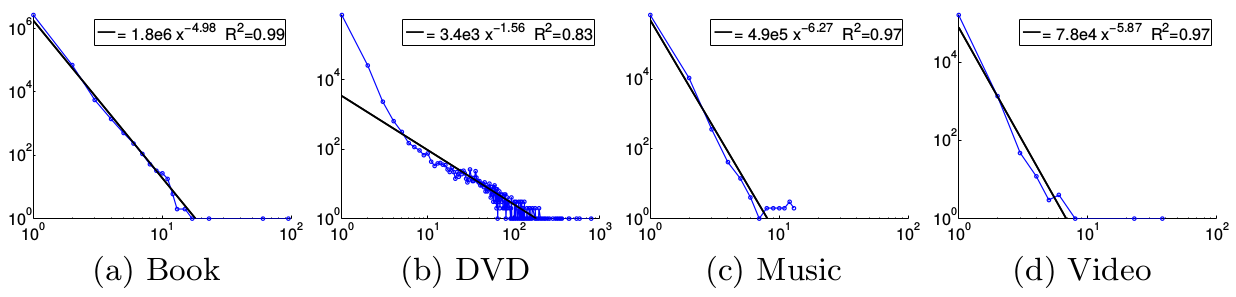
\includegraphics[width=1\textwidth]{figures/rec_cascades_size_count}
				\caption{Size distribution of recommendation cascades for four product categories}
				\small
				This diagram was taken from \citep{RecCascades}, page 7.
				\label{fig:cascade_size_count}
			\end{center}
		\end{figure}
		
		The above analysis holds several insights which in combination lead to a remarkable conclusion:
		
		\begin{enumerate}
			\item The cascades presented in the paper represent only 'successful' recommendations, i.e. the ones which receivers perceived as valuable enough to actually buy the product.
			\item The goal of any recommender algorithm (regardless on which item space it operates) is to produce exactly such valuable recommendations.
			\item Because most cascade sub-graphs were of very small size and degree, 'successful' recommendations can be assumed to originate from places in the direct neighborhood of a node.
		\end{enumerate}
		
		
		\subsection{The local sphere (idea)}
		\label{ssect:the_local_sphere}
		
		The concept of a local sphere and computations applied to it comes from the author's (possibly incorrect, but natural) insight that the relevance of recommendations behaves as a function of node vicinity:
		
		\begin{itemize}
			\item Lets call the whole social graph and all interactions in it the 'global sphere'.
			\item Recommendations to users are then computed over the global sphere, which takes an amount of resources exponential to the size of the underlying graph.
			\item Let's further assume that 95\% of all relevant (accepted) recommendations in a social network like facebook are those that are derived from the immediate local neighborhood of a node (less than 2 degrees, see section above..)
			\item This assumption is corroborated by the fact that two degrees are also what Facebook allows programmers (as of 2013) to query via their graph API from any authenticated user, apparently in an effort to prevent automatic traversal / exploration of their most valuable business asset.
			\item Let's call this immediate local neighborhood the 'local sphere'
		\end{itemize}
			
		Now let's also consider how modern publish/subscribe based frameworks (like Sails, Meteor, Hapi or Derby, only to mention some JavaScript libraries) handle data communication between server and client:
		
		\begin{itemize}
			\item The server offers some subscriptions on it's data, usually limiting access to items based on identity, authorization or user role provided by the client.
			\item The client defines some subscriptions on server-side data collections (tables), representing the client's wish for information regardless of it's status or authority.
			\item Publication as well as subscription can be seen as a mathematical subset of all the data in the database.
			\item An algorithm inside the respective framework resolves those (potentially conflicting) interests by computing the intersection set of the data provided / requested.
			\item The intersection data set is then pushed to the client (in our case the browser) as soon as it becomes available or is updated, which makes this model ideal for real-time interaction and communication between clients.
			\item The sum total of all the data pushed to the client is equivalent to the 'local sphere' we described earlier - HOWEVER - their inherent graph structure is lost during the transmission, so that the client can only see them as isolated fragments without context.
		\end{itemize}
		
		The combination of those two ideas now enables us to envision the following scenario:
		
		\begin{itemize}
			\item Instead of interpreting all data items in the local sphere as isolated entities, we retain their graph structure enabling the client to gain hitherto unachieved knowledge and insights into its already available data.
			\item We therefore need a graph library in the browser, not only to represent the local sphere graph, but also to analyze it in order to take intelligent actions that were previously reserved for the server-side (data center) infrastructure.
			\item No complex graph partitioning algorithm on the server is necessary, as we can use the natural set contraints inherent in any web application:
			\begin{itemize}
				\item e.g. in a social network, the client will have access to all its immediate friends, social activities and interest groups
				\item in a project management tool, the client naturally has access to the data of all team members, to-do lists, milestones, resources etc.
			\end{itemize}
			If our 95\%-relevance assumption mentioned earlier holds, we can achieve great scaling efficiency by introducing the local sphere concept:
			\begin{itemize}
				\item the client can immediately perform computations like recommendations on the subgraph of the local sphere.
				\item only recommendations accepted will have to be stored on the server (that is, cause additional network traffic).
				\item the client is easily able to recompute the relatively small local graphs in real-time, offering responsiveness far beyond today's best (server-side) infrastructures.
				\item as modern web frameworks transport all of the required data into the client store anyways, we do not add extra complexity to our servers and databases.
			\end{itemize}
			\item On the other hand, questions of data security / privacy will have to be dealt with, as we are talking about preemptively filling the client memory with possibly otherwise unnecessary or superfluous data.
		\end{itemize}
		
		
		\begin{figure}[ht]
			\label{fig_local_sphere}
			\begin{center}
				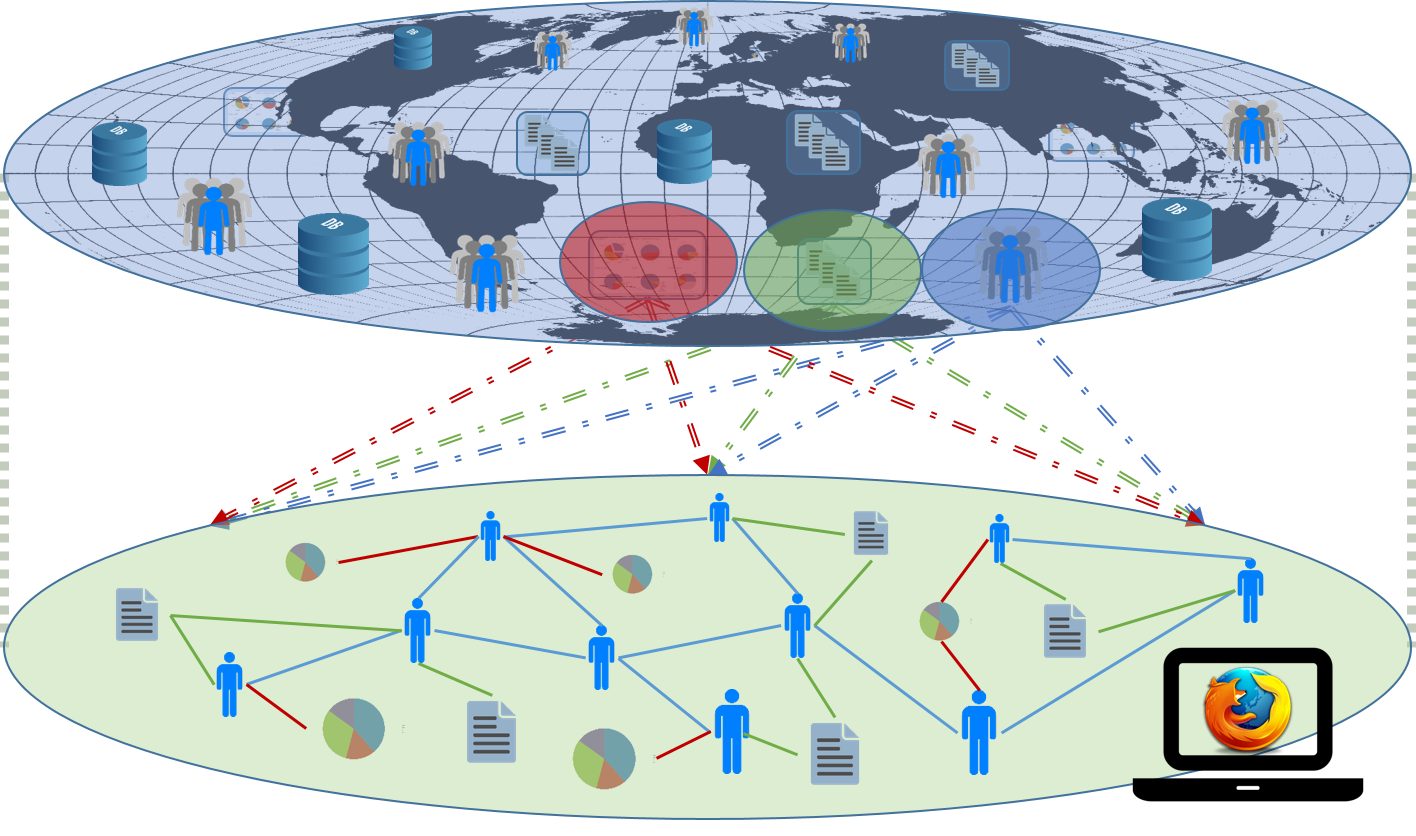
\includegraphics[width=1\textwidth]{figures/local_sphere}
				\caption{Local sphere projected from the global sphere}
			\end{center}
			\small
			Only a very small portion of the global graph is actually visible from any connected client. The sum of all viewable items however, if properly conveyed to the client (i.e. with their connection information preserved), could form a subgraph of the whole network called the 'local sphere', which would allow the browser to utilize the underlying graph structure to extract hidden knowledge and perform graph computations on its own.
		\end{figure}
		
		Needless to say, GraphiniusJS would be an ideal candidate to explore this concept further and could, if used appropriately on carefully modeled local spheres, enable start-ups to compete with much larger companies employing complex and very expensive machine learning infrastructures.
		
	
	\section{Graph based image processing}
	\label{ssect:app_graph_img_proc}
	
	The overall goal of working with images using graph theory contains 3 different aspects: 1) Extracting graphs out of images, thereby laying the groundwork for applying the wealth of graph theory to a hitherto different problem domain, 2) Actually processing the resulting graph with appropriate methods in order to achieve usable (interpretable) results, and 3) visualizing every step of the pipeline, thereby enabling researchers and domain experts to learn valuable lessons from new methods applied. Figure~\ref{fig_graph_based_img_classification} illustrates how a prototypical workflow could look like.
	
	\begin{figure}[ht]
		\begin{center}
			
\includegraphics[width=1\textwidth]{figures/graph_img_class}
			\caption{Graph based image classification example}
			\label{fig_graph_based_img_classification}
		\end{center}
		\small
		1) a laser scan image of a nevus is oversegmented and 2) a graph extracted by interpreting region centroids as nodes and region adjacency as edges. 3) A belief propagation algorithm is applied to the resulting graph yielding 2) a converged state representing the nevus classification as benign or malignant.
	\end{figure}
		
		\subsection{Graph extraction}
		\label{ssect:graph_extraction}
	
		In the attempt to extract graphs out of images, aside from traditional image segmentation approaches \citep{FelzenszwalbHuttenlocher2004}, there have been methods proposed for constructing object graphs from images, e.g. \citep{LeeObjectGraphs2012}. As for the task of merging several extracted graphs into one, we might build upon the work of \citep{Schneevoigt2014}, in which they propose a 3-step pipeline for the reconstruction of 3D objects from 2D image structures by solely utilizing dense methods of correlation analysis (global energy features instead of sparse local feature vectors. For purposes of the latter, \citep{Demetz2013} proposes a new local descriptor called Complete Rank Transform which is morphologically as well as illumination invariant, while containing a maximally possible amount of information \citep{Bobylev2014}. It would be interesting to see if those methods can also be applied to graphs while still retaining sufficient feature information. Moreover, any point cloud data \citep{PointCloudPaper2014} could be interpreted as graphs by enriching them with connections in order to form networks.
		
		\subsection{Graph processing}
		\label{ssect:graph_processing}
		
		\cite{LeeObjectGraphs2012} propose to conduct object recognition based on pre-existing models of known object primitives and to construct object graphs in order to infer global scene understanding from local information.
		
		Another way is to see graphs extracted from image sources as topographic maps. On such "landscapes" autonomous multi-agents \citep{Kasaiezadeh2013MultiagentImage} \citep{Olfati-Saber2007MultiAgents}, e.g. ant-robots \citep{WagnerBruckstein2001FromAntsToAgents} could explore the terrain and leave markings on interesting spots.
		
		From the field of topology, \citep{Cerri2012} describe a method of shape comparison based on Topological Persistence utilizing Persistence Diagrams - collections of shape descriptors - and computing a distance function between them, while \citep{DiFabio2012} applies this idea to shape retrieval by showing partial similarity of such descriptors.
		
		\subsection{Graph visualization}
		\label{ssect:graph_visualization}
		
		As far as visualization is concerned, Graph layouts have been often applied, but because of the scale and complexity of real world data, these layouts tend to be dense and often contain difficult to read edge configurations \citep{HermanMelanconMarshall2000GraphVisIEEE}. Much previous work on graph layouts has focused on algorithmic approaches for the creation of readable layouts and on issues such as edge crossings and bends in layout aesthetics \citep{Purchase1997GraphDrawing}. As an algorithm designer, the decision whether or not to preserve the mental map is more dependent on the tasks likely to be performed by users than previously assumed, however, much further experimentation is needed \citep{ArchambaultPurchase2013MentalMap, StahlGabrys2013GraphbasedKDD}.
		
		In the context of Graphinius (VIS), an additional question presents itself in the form of 3D visualization of large data structures, especially since most layout algorithms to date are specifically limited to 2D projections.
		
		
	% \section{Biomedical applications}
	% \label{sect:app_biomed}
	
	% In the field of 
	% PPI
	% Connectome
	% Metabolics graphs	
	
	
	\section{Anonymization}
	\label{sect:app_snonymization}
	
	The amount of patient-related data produced in today’s clinical setting poses many challenges with respect to collection, storage and responsible use. For example, in research and public health care analysis, data must be anonymized before transfer, for which the k-anonymity measure was introduced and successively enhanced by further criteria like L-diversity, T-closeness as well as delta-presence (the latter of which is used to model the background knowledge of potential attackers).
	
	Taking a look at Figure~\ref{fig:anon_categories} will help the reader in understanding the original (tabular) concept of anonymization: Given an input table with several columns, we will probably encounter three different categories of data:
	
	\begin{itemize}
		\item \textbf{Personal identifiers} are data items which directly identify a person without having to cross-reference or further analyze them. Examples are first and last names, but even more so an (email) address or social security number (SSN). As personal identifiers are dangerous and cannot be generalized (see Figure~\ref{fig:gen_hierarchy}) in a meaningful way (e.g. one could generalize the \textit{address} field, which would only result in some kind of Zip code), this category of data is usually removed. The table shows this column in a red background color.
		\item \textbf{Sensitive data,} also called 'payload', which is the kind of data we want to convey for statistics or research purposes. Examples for this category would be disease classification, drug intake or personal income level. This data shall be preserved in the anonymized dataset and can therefore not be deleted or generalized. The table shows this column in a green background color.
		\item \textbf{Quasi identifiers}, colored in the table with an orange background, are data that in themselves do not directly reveal the identity of a person, but might be used in aggregate to reconstruct it. For instance, \citep{sweeney2002k} mentioned that 87\% of U.S. citizens in 2002 had reported characteristics that made them vulnerable to identification based on just the 3 attributes \textit{zip code}, \textit{gender} and \textit{date of birth}. But although this data can be harmful in that respect, it might also hold vital information for the purpose of research (e.g. zip code could be of high value in a study on disease spread). The solution - and this is the actual point of all anonymization efforts - is to generalize this kind of information, which means to lower its level of granularity. As an example, one could generalize the ZIP codes 41074, 41075 and 41099 to a generalized version 410**, as shown in Figure~\ref{fig:anonymized_clusters}.
	\end{itemize}
	
	\begin{figure}[ht]
		\begin{center}
			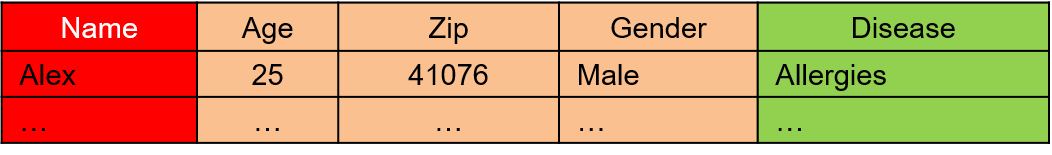
\includegraphics[width=0.9\textwidth]{figures/anonym/3typesofdata}
			\caption{The three types of data considered in (k-)anonymization}
			\label{fig:anon_categories}
		\end{center}
	\end{figure}
	
	As described in \citep{ciriani2007kappa}, k-anonymization requires that in each data release every combination of values of quasi-identifiers must be identical to at least $k-1$ other entries in that release, which can be seen as a clustering problem with each cluster's (in the context of anonymization also called an 'equivalence class') internal quasi-identifier state being identical for every data point. This can be achieved via suppression and generalization, where suppression means simply deletion, whereas in generalization we try to retain some usable value.
	
	The process of generalization works through a concept called \textit{generalization hierarchies}, which form a tree whose root denotes the most general value available for a data category (usually the 'all' value) and then branches to more and more specific occurrences, with its leafs representing the set of exact, original values (see Figure~\ref{fig:gen_hierarchy}). In generalizing some original input value, one traverses the tree from the leaf level upwards until a certain prerequisite is fulfilled. Usually, this prerequisite comes in the form of the k-anonymity requirement, so that we want to find a group of other data rows (=vectors) whose (generalized) quasi identifiers match the data point being processed.
	
	\begin{figure}[ht]
		\begin{center}
			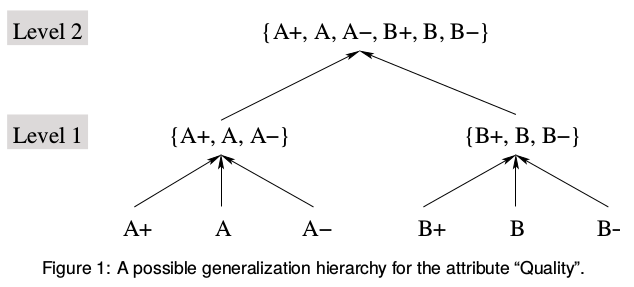
\includegraphics[width=0.8\textwidth]{figures/anonym/gen_hierarchy}
			\caption{Example of a typical generalization hierarchy}
			\label{fig:gen_hierarchy}
			\small
			taken from \citep{aggarwal2005approximation}
		\end{center}
	\end{figure}
	
	
	Each level of generalization involves a certain cost in information loss though, which means we do not just want to construct our clusters in any sequence possible, but minimize the overall information loss. This makes k-anonymization an NP-hard optimization problem (because of an exponential number of possible generalized quasi-identifier combinations), leaving us to conclude that the k-Anonymity problem is to lose as little information as possible in a dataset while ensuring that the release (the anonymized, publishable version of the dataset) satisfies the k-anonymization criterion \citep{aggarwal2005approximation}.
	
	\begin{figure}[H]
		\centering
		\begin{minipage}[b]{0.5\textwidth}
			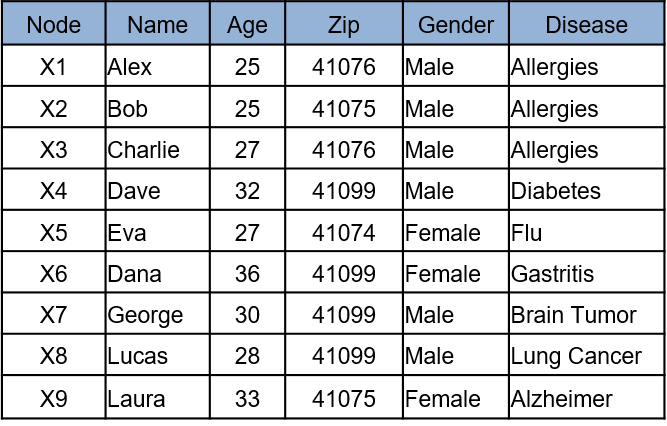
\includegraphics[width=\textwidth]{figures/anonym/k_anon_input}
		\end{minipage}
		\hfill
		\begin{minipage}[b]{0.418\textwidth}
			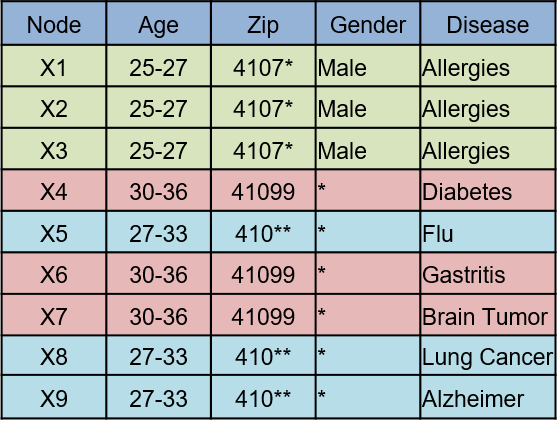
\includegraphics[width=\textwidth]{figures/anonym/k_anon_output}
		\end{minipage}
		\caption{Tabular anonymization: input table and anonymization result}
		\label{fig:anonymized_clusters}
	\end{figure}
	
	
	\section{Graph (social network) anonymization}
	\label{sect:graph_sn_anon}
	
	The whole last sections would have been out of place in a thesis regarding a graph platform and library, as it holds no direct references to graph computations. However, as social networks have gained huge popularity over the previous decade, and even modern medical databases come in the form of graph structures, the question of how to efficiently anonymize networks has gained ever more significance over the years.
	
	As a start, one could see a graph just as a collection of nodes, where each node contains some kind of feature vector, akin to the row in a data table. Adopting that view, we could be tempted to simply ignore the existence of edges and apply some kind of algorithm suitable to the anonymization of tabular data. The main problem with this however lies in the fact that the structural environment of a node (the constellation of its neighbors within the greater network) provides some additional information. That is, even if we successfully (k-)anonymize the feature vectors of a graph according to the methods found in the previous chapter, we still run the risk of leaving to much information in the form of a known local subgraph structure.
	
	Consider Figure~\ref{fig:anon_sn_problem} for example, in which the nodes of a graph have already been k-anonymized into groups of size 3 and 7, respectively. In this figure, local subgraphs b) and c) are actually (3)-anonymized, because as each node has the exact same local neighborhood structure, the additional information of a node possessing a degree of 0 (or 2) is of no additional value. For local subgraphs a) and d) on the other hand, the additional information of a node being of degree (x) has the potential to reveal its identity, as it is not indistinguishable from its neighbors within the equivalence class any more.
	
	\begin{figure}[ht]
		\begin{center}
			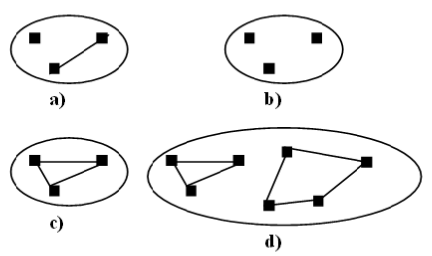
\includegraphics[width=0.8\textwidth]{figures/anonym/sn_problem}
			\caption{Local subgraph neighborhoods as additional anonymization obstacle.}
			\label{fig:anon_sn_problem}
		\end{center}
		\small
		(Example taken from \cite{campan2009data}.)
	\end{figure}
	
	Several methods have been proposed to make re-identification of nodes in anonymized social graphs harder.	\cite{chester2011k} for example introduce the idea of vertex addition to labeled and unlabeled datasets. While an algorithm on the former remains NP complete, they provide an efficient ($O(nk)$) algorithm for unlabeled data. Experimenting on several well known datasets, they show that commonly-studied structural properties of the network, such as clustering coefficient, are only minorly distorted by their anonymization procedure.
	
	The authors of \citep{kapron2011social} take the approach of adding edges to an edge-labeled graph like the Netflix movie database (with users and movies being nodes and edge weights representing movie ratings). They define tables as bipartite graphs and prove NP-hardness for the problems of neighborhood anonymity, i-hop anonymity and k-symmetry anonymity.
	
	\cite{campan2009data}, whose local subgraph problem we already encountered, proposed a solution in the form of a greedy clustering algorithm which takes into account not only the information loss incurred by generalizing features of nodes, but also introducing a structural loss function based on the local neighborhood within an equivalence class (and between them). The author of this thesis implemented that approach utilizing GraphiniusJS and will demonstrate the algorithm in Section~\ref{sect:aoa_anonymization} as well as the anonymized results in Appendix Section~\ref{sect:anon_output_data}.		
	
	
	\section{Fraud detection}
	\label{sect:fraud_detection}

	Anomaly detection via belief propagation in a Markov random field (BP-MRF) has been shown to work on large networks with high accuracy and realistic performance \citep{BeliefPropFraudDetection2007}, and can also be adapted to scale to hundreds of parallel machines as described in \citep{BeliefPropBillionNodes2010}.
	
	The idea behind this approach is that each node in a graph holds some belief about itself and is capable of forming opinions of its neighbors. Let's assume a group of people represented by nodes and edges denoting friendships between those nodes; let's further assume that a small subgroup of people are criminals and that criminals usually engage in friendship with other criminals, while non-criminals prefer to stay amongst themselves as well. 
	
	Given this model we can infer that if a node has a lot of edges to criminals, there is a higher chance for the underlying person to be a criminal as well. We first initialize this system with a certain belief structure (some nodes believe they are criminals, others don't) and we let nodes form opinions about each other ("you are connected to me and I am a criminal, therefore you must be a criminal also"). If we subsequently initiate a turn-based exchange of those opinions with a slight chance per turn of "convincing" a neighboring node, that system might (but not necessarily has to) converge to a stable state - a final belief distribution about who is a criminal and who is not.
	
	Although the example given might sound exotic at first, Belief Propagation has already successfully been applied to email spam classification and fraud detection in auction systems in 2007, improving the methods previously employed by significant margins.
